\documentclass{beamer}

\pdfmapfile{+sansmathaccent.map}


\mode<presentation>
{
	\usetheme{Warsaw} % or try Darmstadt, Madrid, Warsaw, Rochester, CambridgeUS, ...
	\usecolortheme{seahorse} % or try seahorse, beaver, crane, wolverine, ...
	\usefonttheme{serif}  % or try serif, structurebold, ...
	\setbeamertemplate{navigation symbols}{}
	\setbeamertemplate{caption}[numbered]
} 


%%%%%%%%%%%%%%%%%%%%%%%%%%%%
% itemize settings

\definecolor{mypaleblue}{RGB}{240, 240, 255}
\definecolor{mylightblue}{RGB}{120, 150, 255}
\definecolor{myblue}{RGB}{90, 90, 255}
\definecolor{mygblue}{RGB}{70, 110, 240}
\definecolor{mydarkblue}{RGB}{0, 0, 180}
\definecolor{myblackblue}{RGB}{40, 40, 120}

\definecolor{mygreen}{RGB}{0, 200, 0}
\definecolor{mydarkgreen}{RGB}{0, 120, 0}
\definecolor{mygreen2}{RGB}{245, 255, 230}

\definecolor{mygray}{gray}{0.8}
\definecolor{mygray2}{RGB}{130, 130, 130}
\definecolor{mydarkgray}{RGB}{80, 80, 160}
\definecolor{mylightgray}{RGB}{160, 160, 160}

\definecolor{mydarkred}{RGB}{160, 30, 30}
\definecolor{mylightred}{RGB}{255, 150, 150}
\definecolor{myred}{RGB}{200, 110, 110}
\definecolor{myblackred}{RGB}{120, 40, 40}

\definecolor{mypink}{RGB}{255, 30, 80}
\definecolor{myhotpink}{RGB}{255, 80, 200}
\definecolor{mywarmpink}{RGB}{255, 60, 160}
\definecolor{mylightpink}{RGB}{255, 80, 200}
\definecolor{mydarkpink}{RGB}{155, 25, 60}

\definecolor{mydarkcolor}{RGB}{60, 25, 155}
\definecolor{mylightcolor}{RGB}{130, 180, 250}

\setbeamertemplate{itemize items}[default]

\setbeamertemplate{itemize item}{\color{myblackblue}$\blacksquare$}
\setbeamertemplate{itemize subitem}{\color{mydarkblue}$\blacktriangleright$}
\setbeamertemplate{itemize subsubitem}{\color{mygray}$\blacksquare$}

\setbeamercolor{palette quaternary}{fg=white,bg=mygblue} %mydarkgray
\setbeamercolor{titlelike}{parent=palette quaternary}

\setbeamercolor{palette quaternary2}{fg=white,bg=mygblue}%black myblue
\setbeamercolor{frametitle}{parent=palette quaternary2}

\setbeamerfont{frametitle}{size=\Large,series=\scshape}
\setbeamerfont{framesubtitle}{size=\normalsize,series=\upshape}


%%%%%%%%%%%%%%%%%%%%%%%%%%%%
% block settings

%\setbeamercolor{block title}{bg=red!50,fg=black}
%\setbeamercolor{block title}{bg=mylightblue,fg=black}
\setbeamercolor{block title}{bg=myblackblue,fg=white}

\setbeamercolor*{block title example}{bg=mygreen!40!white,fg=black}

\setbeamercolor*{block body example}{fg= black,
	bg= mygreen2}


%%%%%%%%%%%%%%%%%%%%%%%%%%%%
% URL settings
\hypersetup{
	colorlinks=false,
	linkcolor=blue,
	filecolor=blue,      
	urlcolor=blue,
}

%%%%%%%%%%%%%%%%%%%%%%%%%%

\renewcommand{\familydefault}{\rmdefault}

\usepackage{amsmath}
\usepackage{mathtools}

\usepackage{subcaption}

\usepackage{qrcode}

\newcommand{\bo}[1] {\mathbf{#1}}
\newcommand{\R}{\mathbb{R}} 
\newcommand{\T}{^\top}     



\newcommand{\mydate}{Spring 2025}

\newcommand{\mygit}{\textcolor{blue}{\href{https://github.com/SergeiSa/Computational-Intelligence-2025}{github.com/SergeiSa/Computational-Intelligence-2025}}}

\newcommand{\myqr}{ \textcolor{black}{\qrcode[height=1.5in]{https://github.com/SergeiSa/Computational-Intelligence-2025}}
}

\newcommand{\myqrframe}{
	\begin{frame}
		\centerline{Lecture slides are available via Github, links are on Moodle:}
		\bigskip
		\centerline{\mygit}
		\bigskip
		\myqr
	\end{frame}
}


\newcommand{\bref}[2] {\textcolor{blue}{\href{#1}{#2}}}



%%%%%%%%%%%%%%%%%%%%%%%%%%%%
% code settings

\usepackage{listings}
\usepackage{color}
% \definecolor{mygreen}{rgb}{0,0.6,0}
% \definecolor{mygray}{rgb}{0.5,0.5,0.5}
\definecolor{mymauve}{rgb}{0.58,0,0.82}
\lstset{ 
	backgroundcolor=\color{white},   % choose the background color; you must add \usepackage{color} or \usepackage{xcolor}; should come as last argument
	basicstyle=\footnotesize,        % the size of the fonts that are used for the code
	breakatwhitespace=false,         % sets if automatic breaks should only happen at whitespace
	breaklines=true,                 % sets automatic line breaking
	captionpos=b,                    % sets the caption-position to bottom
	commentstyle=\color{mygreen},    % comment style
	deletekeywords={...},            % if you want to delete keywords from the given language
	escapeinside={\%*}{*)},          % if you want to add LaTeX within your code
	extendedchars=true,              % lets you use non-ASCII characters; for 8-bits encodings only, does not work with UTF-8
	firstnumber=0000,                % start line enumeration with line 0000
	frame=single,	                   % adds a frame around the code
	keepspaces=true,                 % keeps spaces in text, useful for keeping indentation of code (possibly needs columns=flexible)
	keywordstyle=\color{blue},       % keyword style
	language=Octave,                 % the language of the code
	morekeywords={*,...},            % if you want to add more keywords to the set
	numbers=left,                    % where to put the line-numbers; possible values are (none, left, right)
	numbersep=5pt,                   % how far the line-numbers are from the code
	numberstyle=\tiny\color{mygray}, % the style that is used for the line-numbers
	rulecolor=\color{black},         % if not set, the frame-color may be changed on line-breaks within not-black text (e.g. comments (green here))
	showspaces=false,                % show spaces everywhere adding particular underscores; it overrides 'showstringspaces'
	showstringspaces=false,          % underline spaces within strings only
	showtabs=false,                  % show tabs within strings adding particular underscores
	stepnumber=2,                    % the step between two line-numbers. If it's 1, each line will be numbered
	stringstyle=\color{mymauve},     % string literal style
	tabsize=2,	                   % sets default tabsize to 2 spaces
	title=\lstname                   % show the filename of files included with \lstinputlisting; also try caption instead of title
}

%%%%%%%%%%%%%%%%%%%%%%%%%%%%
% tikz settings

\usepackage{tikz}
\tikzset{every picture/.style={line width=0.75pt}}

%%%%%%%%%%%%%%%%%%%%%%%%%%%%




\title{Second-order cone programming}
\subtitle{Computational Intelligence, Lecture 9}
\author{by Sergei Savin}
\centering
\date{\mydate}



\begin{document}
\maketitle


\begin{frame}{Content}

\begin{itemize}
	\item  Norm
\item  Second-order cone programming
\item  SOCP to QCQP
\item  Friction cone as an SOCP
\end{itemize}

\end{frame}






\begin{frame}{2-norm, 1}
	% \framesubtitle{Parameter estimation}
	\begin{flushleft}
		
		Let us consider a 2-norm as a function $f(\bo{x}): \ \R^n \rightarrow \R$:
		
		\begin{align}
			f(\bo{x}) = || \bo{x} ||_2
			\\
			f(\bo{x}) = \sqrt{ \sum_{i=1}^n x_i^2 }
		\end{align}
		
	\end{flushleft}
\end{frame}


\begin{frame}{2-norm, 2}
	% \framesubtitle{Parameter estimation}
	\begin{flushleft}
		
		We can describe 2-norm as a surface in the $\mathcal S \subset \R^{n+1}$ space:
		
		\begin{align}
			\mathcal S = \{  (J, \bo{x}): \ J = || \bo{x} ||_2 \}
		\end{align}		
		
		% TODO: \usepackage{graphicx} required
		\begin{figure}
			\centering
			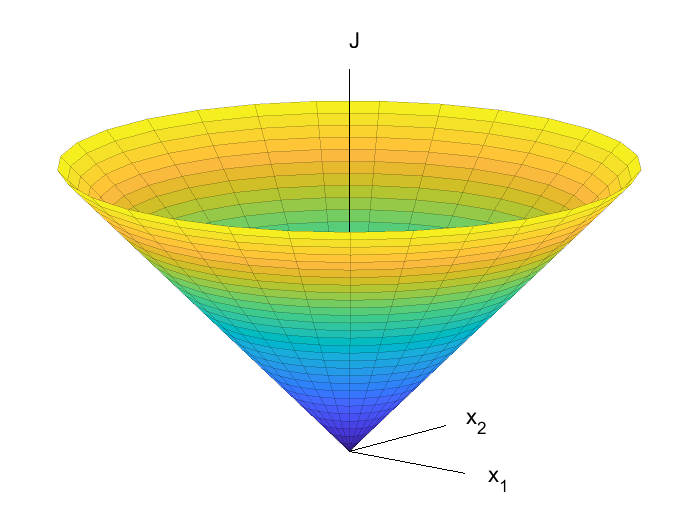
\includegraphics[width=0.7\linewidth]{norm}
			%			\caption{}
			\label{fig:norm}
		\end{figure}
		
	\end{flushleft}
\end{frame}



\begin{frame}{Cone}
	% \framesubtitle{Parameter estimation}
	\begin{flushleft}
		
		The shape of the surface $\mathcal S = \{  (J, \bo{x}): \ J = || \bo{x} ||_2 \}$ is a \emph{cone}. We observe the following properties of a cone:
		
		\begin{itemize}
			\item There is a single tip point $\tau$ and a normal direction.
			
			\item  Slicing cone with planes orthogonal to the normal direction, we produce ellipsoids (we can call it tangent sets).
			
			\item For any point $p$ on the cone, the half-line from the tip point $\tau$ through $p$ lies on the cone. The angle between this line and the normal is called \emph{vertex angle}.
		\end{itemize}
		
		%\bigskip
		
		%The tip point for $\mathcal S$ is $(0, \bo{0})$. Normal direction is $(n, \bo{0})$. Tangent sets are circles $|| \bo{x} ||_2 = h$, parameterized by $h$. 
		
		%For any point $(J(\bo{p}), \bo{p})$ we can write half-line as $\mathcal L = \{ ( J(\gamma \bo{p}), \gamma \bo{p}): \ \gamma > 0 \}$.
		
		%\begin{align}
			%J(\gamma \bo{p}) = ||\gamma \bo{p}|| = \gamma ||\bo{p}|| = \gamma J(\bo{p})
		%\end{align}
		
	\end{flushleft}
\end{frame}







\begin{frame}{Second-order cone}
	% \framesubtitle{Parameter estimation}
	\begin{flushleft}
		
		A second-order cone constraint has the following form:
		
		\begin{equation}
			||\bo{A}\bo{x}+\bo{b}|| \leq \bo{c}\T \bo{x} + d
		\end{equation}
		%
		where $\bo{A} \in \R^{n, n}$, $\bo{b}, \bo{c} \in \R^{n}$ and $d \in \R$.
		
		\bigskip
		
		This constraint describes interior of a cone. The surface of the cone is an intersection of two surfaces: 
		
		\begin{align}
			J = ||\bo{A}\bo{x}+\bo{b}|| \\
			P = \bo{c}\T \bo{x} + d
		\end{align}
		
		First is a cone and second is a plane. Their intersection is called a \emph{conic section}. 
		
		
	\end{flushleft}
\end{frame}






\begin{frame}{The role of the free constant, 1}
	% \framesubtitle{Parameter estimation}
	\begin{flushleft}
		
		Typical conic sections are shown below:
		
		% TODO: \usepackage{graphicx} required
		\begin{figure}
			\centering
			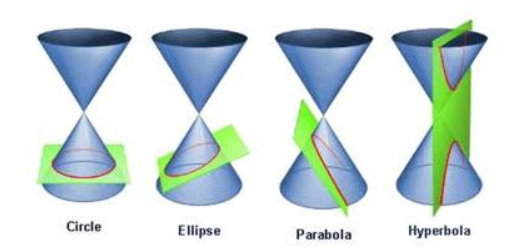
\includegraphics[width=0.7\linewidth]{cones}
			\label{fig:cones}
		\end{figure}
		
		As we can see, they represent ellipsoid and parabola. In order for them to represent a cone, the plane  $S$ needs to pass through the tip of the cone $J$. This can be achieved with the appropriate choice of constant $d$, which shifts $S$ up or down.
		
	\end{flushleft}
\end{frame}



\begin{frame}{The role of the free constant, 2}
	% \framesubtitle{Parameter estimation}
	\begin{flushleft}
		
		The surface of a second-order cone (SOC) is:
		%
		\begin{equation}
			||\bo{A}\bo{x}+\bo{b}|| = \bo{c}\T \bo{x} + d
		\end{equation}
		
		we can find a tip point; it corresponds to both right-hand side and left-hand side becoming zero:
		
		\begin{equation}
			\begin{cases}
				\bo{A}\bo{x}+\bo{b} = 0 \\
				\bo{c}\T \bo{x} + d = 0
			\end{cases}
		\end{equation}
		
		Given full rank matrix $\bo{A}$, the solution is $\bo{x} = -\bo{A}^{-1}\bo{b}$. The system would hold if:
		
		\begin{equation}
			-\bo{c}\T \bo{A}^{-1}\bo{b} + d = 0
		\end{equation}
		
		
	\end{flushleft}
\end{frame}







\begin{frame}{Second-order cone programming (SOCP)}
\framesubtitle{General form}
\begin{flushleft}


The general form of a Second-order cone program (SOCP) is:

%
\begin{equation}
\begin{aligned}
& \underset{\mathbf{x}}{\text{minimize}}
& & \mathbf{f}^\top\mathbf{x}, \\
& \text{subject to}
& & \begin{cases}
    ||\mathbf{A}_i\mathbf{x} + \mathbf{b}_i||_2 \leq 
     \mathbf{c}_i^\top \mathbf{x} + d_i, \\
    \mathbf{F}\mathbf{x} = \bo{g}.
    \end{cases}
\end{aligned}
\end{equation}

LP, QP and QCQP are subsets of SOCP.
 
\end{flushleft}
\end{frame}








\begin{frame}{Second-order cone programming}
\framesubtitle{Special cases}
\begin{flushleft}

We can write problem where our domain is a ball as SOCP:
%
\begin{equation}
\begin{aligned}
& \underset{\mathbf{x}}{\text{minimize}}
& & \mathbf{f}^\top\mathbf{x}, \\
& \text{subject to}
& & ||\mathbf{x}||_2 \leq d_i
\end{aligned}
\end{equation}

\bigskip

Same for ellipsoidal constraints:
%
\begin{equation}
\begin{aligned}
& \underset{\mathbf{x}}{\text{minimize}}
& & \mathbf{f}^\top\mathbf{x}, \\
& \text{subject to}
& & ||\mathbf{A}_i\mathbf{x}||_2 \leq d_i
\end{aligned}
\end{equation}
 
\end{flushleft}
\end{frame}




\begin{frame}{Example - path planning}
	\begin{flushleft}
		
		Consider a path planning problem: find a sequence of points $\bo{x}_i$ starting at $\bo{x}_0$, making a shortest path to the goal point $\bo{x}_g$, such that neightbouring points are no further than $h$ from one another.
		
		\bigskip
		
		\textbf{Solution}. 
		The problem becomes:
		
		
		%
		\begin{equation}
			\begin{aligned}
				& \underset{\bo{x}_1, ..., \bo{x}_n}{\text{minimize}}
				& & \sum_{i = 1}^{n} (\bo{x}_i - \bo{x}_g)\T (\bo{x}_i - \bo{x}_g), \\
				& \text{subject to}
				& &||\bo{x}_i - \bo{x}_{i+1} || < h, \ \ i \in {0, 1, 2, ...., n}
			\end{aligned}
		\end{equation}
		
	\end{flushleft}
\end{frame}




\begin{frame}{SOCP to QCQP, 1}
% \framesubtitle{Part 1}
\begin{flushleft}

Set $\mathbf{c}_i = 0$ and recognize that $||\mathbf{A}_i\mathbf{x} + \mathbf{b}_i||_2 \leq d_i$ is the same as $(\mathbf{A}_i\mathbf{x} + \mathbf{b}_i)^\top (\mathbf{A}_i\mathbf{x} + \mathbf{b}_i) \leq d_i^2$ (since the first implies that $d_i$ is non-negative).

\bigskip
%
\begin{equation}
\begin{aligned}
& \underset{\bo{x}}{\text{minimize}}
& & \bo{f}^\top\bo{x}, \\
& \text{subject to}
& & \begin{cases}
    \bo{x}^\top \bo{A}_i^\top \bo{A}_i \bo{x} + 
    2 \bo{b}_i^\top \bo{A}_i\bo{x} + 
    \bo{b}_i^\top \bo{b}_i  \leq d_i^2\\
    \bo{F}\bo{x} = \bo{g}.
    \end{cases}
\end{aligned}
\end{equation}

\end{flushleft}
\end{frame}




\begin{frame}{SOCP to QCQP, 2}
%\framesubtitle{Part 2}
\begin{flushleft}


Now to make the cost quadratic:
%
\begin{equation}
\begin{aligned}
& \underset{\bo{x}, t}{\text{minimize}}
& & t, \\
& \text{subject to}
& & \begin{cases}
    \bo{x}^\top \bo{A}_0^\top \bo{A}_0 \bo{x} + 
    2 \bo{b}_0^\top \bo{A}_0\bo{x} + 
    \bo{b}_0^\top \bo{b}_0  \leq t\\
    \bo{x}^\top \bo{A}_i^\top \bo{A}_i \bo{x} + 
    2 \bo{b}_i^\top \bo{A}_i\bo{x} + 
    \bo{b}_i^\top \bo{b}_i  \leq d_i^2\\
    \bo{F}\bo{x} = \bo{g}.
    \end{cases}
\end{aligned}
\end{equation}

Which is the same as:
%
\begin{equation}
\begin{aligned}
& \underset{\bo{x}}{\text{minimize}}
& & \mathbf{x}^\top \mathbf{H} \mathbf{x} + \mathbf{f}^\top\mathbf{x}, \\
& \text{subject to}
& & \begin{cases}
    \bo{x}^\top \bo{A}_i^\top \bo{A}_i \bo{x} + 
    2 \bo{b}_i^\top \bo{A}_i\bo{x} + 
    \bo{b}_i^\top \bo{b}_i  \leq d_i^2\\
    \bo{F}\bo{x} = \bo{g}.
    \end{cases}
\end{aligned}
\end{equation}

As long as $\bo{A}_0 = \sqrt{\bo{H}}$, and $\bo{b}_0 = 0.5 \bo{A}_0^{-1} \mathbf{f}$.

\end{flushleft}
\end{frame}





\begin{frame}
	\centerline{\huge Friction cone as an SOC}
\end{frame}


\begin{frame}{Friction in 3D, 1}
	% \framesubtitle{Parameter estimation}
	\begin{flushleft}
		
		Friction force $\bo{f}_\tau$ together with normal reaction force $\bo{f}_n$ together form contact reaction force $\bo{f}_R$:
		
		\begin{align}
			\bo{f}_R = \bo{f}_n + \bo{f}_\tau
		\end{align}
		
		We can choose to represent the reaction force in a basis $\bo{B}$ formed by concatenating normal direction $\bo{n}$ and two tangent directions $\bo{t}_1$, $\bo{t}_2$.
		
		\begin{align}
			\bo{f}_R
			=
			\bo{B}
			\begin{bmatrix}
				f_n \\ f_{\tau, 1} \\ f_{\tau, 2}
			\end{bmatrix}
			=
			\begin{bmatrix}
				\bo{n} & \bo{t}_1 & \bo{t}_2
			\end{bmatrix}
			\begin{bmatrix}
				f_n \\ f_{\tau, 1} \\ f_{\tau, 2}
			\end{bmatrix}
		\end{align}
		
		
		
	\end{flushleft}
\end{frame}



\begin{frame}{Friction in 3D, 2}
	% \framesubtitle{Parameter estimation}
	\begin{flushleft}
		
		We can prove that $f_n = \bo{n}\T \bo{f}_R$:
		
		\begin{align}
			\bo{n}\T \bo{f}_R = 
			\bo{n}\T
			\begin{bmatrix}
				\bo{n} & \bo{t}_1 & \bo{t}_2
			\end{bmatrix}
			\begin{bmatrix}
				f_n \\ f_{\tau, 1} \\ f_{\tau, 2}
			\end{bmatrix}
			=
			\begin{bmatrix}
				1 & 0 & 0
			\end{bmatrix}
			\begin{bmatrix}
				f_n \\ f_{\tau, 1} \\ f_{\tau, 2}
			\end{bmatrix}
			=
			f_n 
		\end{align}
		
		
		We can prove that $\begin{bmatrix}
			f_{\tau, 1} \\ f_{\tau, 2}
		\end{bmatrix} = 
		\begin{bmatrix}
			\bo{t}_1 & \bo{t}_2
		\end{bmatrix}\T \bo{f}_R$:
		
		\begin{align}
			\begin{bmatrix}
				\bo{t}_1 & \bo{t}_2
			\end{bmatrix}\T \bo{f}_R = 
			\begin{bmatrix}
				\bo{t}_1 & \bo{t}_2
			\end{bmatrix}\T
			\begin{bmatrix}
				\bo{n} & \bo{t}_1 & \bo{t}_2
			\end{bmatrix}
			\begin{bmatrix}
				f_n \\ f_{\tau, 1} \\ f_{\tau, 2}
			\end{bmatrix}
			= \\
			=
			\begin{bmatrix}
				0 & 1 & 0 \\
				0 & 0 & 1
			\end{bmatrix}
			\begin{bmatrix}
				f_n \\ f_{\tau, 1} \\ f_{\tau, 2}
			\end{bmatrix}
			=
			\begin{bmatrix}
				f_{\tau, 1} \\ f_{\tau, 2}
			\end{bmatrix}
		\end{align}
		
		
	\end{flushleft}
\end{frame}




\begin{frame}{Friction cone representations, 1}
	% \framesubtitle{Parameter estimation}
	\begin{flushleft}
		
		We can write friction cone constraint as follows:
		
		\begin{equation}
			\sqrt{f_{\tau, 1}^2 + f_{\tau, 2}^2} \leq \mu f_n
		\end{equation}
		
		where $\mu$ is friction coefficient, $f_\tau$ is the magnitude of the friction force and $f_n$ is the magnitude of the normal reaction force.
		
		\bigskip
		
		We can describe it as \emph{element-wise description}. The simplicity of this description makes it quite attractive.
		
		
	\end{flushleft}
\end{frame}


\begin{frame}{Friction cone representations, 2}
	% \framesubtitle{Parameter estimation}
	\begin{flushleft}
		
		It is possible to re-write the same constraint as:
		
		\begin{equation}
			\left|\left| \begin{bmatrix}
				\bo{t}_1 & \bo{t}_2
			\end{bmatrix}\T
			\bo{f}_R \right|\right| 
			\leq \mu \bo{n}\T \bo{f}_R
		\end{equation}
		
		We can call it a \emph{vector description}. The advantage of this description is the use of a single vector variable $\bo{f}_R$. It takes the form of a second-order cone (SOC) constraint.
		
		\bigskip
		
		Note that $\bo{t}_1$ and $\bo{t}_2$ are usually not given, and can be chosen arbitrarily, up to rotation. We can find them as a left null space of the normal vector: $\bo{T} = \begin{bmatrix}
			\bo{t}_1 & \bo{t}_2
		\end{bmatrix} = \text{null}(\bo{n}\T)$: 
		
		\begin{equation}
			|| \bo{T}\T\bo{f}_R ||
			\leq \mu \bo{n}\T \bo{f}_R
		\end{equation}
		
	\end{flushleft}
\end{frame}



\begin{frame}{Friction cone representations, 3}
	% \framesubtitle{Parameter estimation}
	\begin{flushleft}
		
		We can do the same with projectors:
		
		
		\begin{equation}
			|| (\bo{I} - \bo{n}\bo{n}\T) \bo{f}_R ||
			\leq \mu \bo{n}\T \bo{f}_R
		\end{equation}
		
		
		
	\end{flushleft}
\end{frame}




\begin{frame}{Homework}
% \framesubtitle{Parameter estimation}
\begin{flushleft}

Plot a cone from a given direction and a given vertex angle.

\end{flushleft}
\end{frame}





\myqrframe



\begin{frame}
	\centerline{\huge Appendix A - canonical form}
\end{frame}


\begin{frame}{Canonical form, degenerate cone marix, 1}
	%	\framesubtitle{General form}
	\begin{flushleft}
		
		Consider the following SOC constraint:
		
		\begin{equation}
			\label{eq:SOC}
			||\mathbf{A}\mathbf{x} + \mathbf{b}||_2 \leq 
			\mathbf{c}^\top \mathbf{x} + d
		\end{equation}
		
		Let us consider a special case when $\mathbf{x} \in \R^n$, $\mathbf{A} \in \R^{(n-1) \times n}$ and $\text{rank}\left(\begin{bmatrix}
			\mathbf{A} \\ \mathbf{c}^\top
		\end{bmatrix}\right) = n$. Then we can introduce the following substitution:
		
		\begin{equation}
			\xi = \begin{bmatrix}
				\mathbf{A} \\ \mathbf{c}^\top
			\end{bmatrix}
			\mathbf{x} + 
			\begin{bmatrix}
				\mathbf{b} \\ d
			\end{bmatrix}, 
			\ \ \ 
			\mathbf{I} = 
			\begin{bmatrix}
				\mathbf{E} \\ \mathbf{e}^\top
			\end{bmatrix}
		\end{equation}
		%
		where $\mathbf{I} \in\R^{n, n}$ is an identity matrix. Then constraint \eqref{eq:SOC} becomes:
		
		\begin{equation}
			||\mathbf{E}\xi||_2 \leq 
			\mathbf{e}^\top \xi
		\end{equation}
		
	\end{flushleft}
\end{frame}


\begin{frame}{Canonical form, degenerate cone marix, 2}
	%	\framesubtitle{General form}
	\begin{flushleft}
		
		Notice that $||\mathbf{E}\xi||_2 \leq 
		\mathbf{e}^\top \xi$ is equivalent to:
		
		\begin{equation}
			\sum\limits_{i=1}^{n-1}\xi_i^2 \leq \xi_n^2 
		\end{equation}
		%	
		which is a standard form of a cone. A map back from $\xi$ to $\mathbf{x}$ is given as:
		
		\begin{equation}
			\mathbf{x} = \begin{bmatrix}
				\mathbf{A} \\ \mathbf{c}^\top
			\end{bmatrix}^{-1}
			\left(
			\xi - 
			\begin{bmatrix}
				\mathbf{b} \\ d
			\end{bmatrix}
			\right)
		\end{equation}
		
	\end{flushleft}
\end{frame}



\begin{frame}
	\centerline{\huge Appendix B - plotting cones}
\end{frame}


\begin{frame}{Plotting level sets, 1}
	% \framesubtitle{Parameter estimation}
	\begin{flushleft}
		
		To plot a cone it is convenient to first use change of coordinates $\bo{y} = \bo{A}\bo{x}+\bo{b}$, meaning $\bo{x} =\bo{A}^{-1} (\bo{y} - \bo{b})$, giving us SOC:
		%
		\begin{equation}
			||\bo{y}|| = \bo{c}\T \bo{A}^{-1} (\bo{y} - \bo{b}) + d
		\end{equation}
		
		Note that $d - \bo{c}\T \bo{A}^{-1}\bo{b} = 0$ for a cone with a tip; so SOC becomes:
		%
		\begin{equation}
			||\bo{y}|| = \bo{c}\T \bo{A}^{-1} \bo{y}
		\end{equation}
		
		To plot level sets of this cone we choose height of the level set $h$ and pick point $\bo{y}_h = h \frac{\bo{A}^{-T} \bo{c}}{\bo{c}\T \bo{A}^{-1}\bo{A}^{-T} \bo{c}}$; we note that $\bo{c}\T \bo{A}^{-1} \bo{y}_h = h$. Then we consider points on the plane $\mathcal P$ orthogonal to $\bo{c}\T \bo{A}^{-1}$ and passing through $\bo{y}_h$:
		
		\begin{equation}
			\mathcal P = {\bo{y}_h + \bo{T}\bo{z}: \  \forall \bo{z}}
		\end{equation}
		%
		where $\bo{T} = \text{null}(\bo{c}\T \bo{A}^{-1})$, so $\bo{c}\T \bo{A}^{-1} \bo{T} = 0$.
		
	\end{flushleft}
\end{frame}


\begin{frame}{Plotting level sets, 2}
	% \framesubtitle{Parameter estimation}
	\begin{flushleft}
		
		Since  SOC becomes:
		%
		\begin{equation}
			||\bo{y}_h + \bo{T}\bo{z}|| = h
		\end{equation}
		
		Since $\bo{y}_h$ and $\bo{T}\bo{z}$ are orthogonal, it is equivalent to:
		%
		\begin{equation}
			||\bo{T}\bo{z}|| = g
		\end{equation}
		%
		where $g = \sqrt{ h^2 - \bo{y}_h\T\bo{y}_h }$. In the 3D case, this is a circle with radius $g$. We can find $N$ consecutive evenly spaced points of this circle, resulting in the next sequence of $\bo{y}_l$:
		
		\begin{align}
			\bo{y}_l &= \bo{y}_h + \bo{T}
			\begin{bmatrix}
				g\cos(\varphi) \\ -g\sin(\varphi)
			\end{bmatrix}, \ \ \ \varphi = 0, \ \frac{2\pi}{N},\ 2\frac{2\pi}{N}, \ ..., \ 2\pi 
			\\
			\bo{x}_l  &=\bo{A}^{-1} (\bo{y}_l - \bo{b})
		\end{align}
		
		The center of the ellipsoid representing this level set lies at the point $\bo{x} =\bo{A}^{-1} (\bo{y}_h - \bo{b})$.
		
	\end{flushleft}
\end{frame}



\begin{frame}{Plotting level sets, 3}
	% \framesubtitle{Parameter estimation}
	\begin{flushleft}
		
		
		\begin{figure}
			\centering
			\begin{subfigure}[b]{0.45\textwidth}
				\centering
				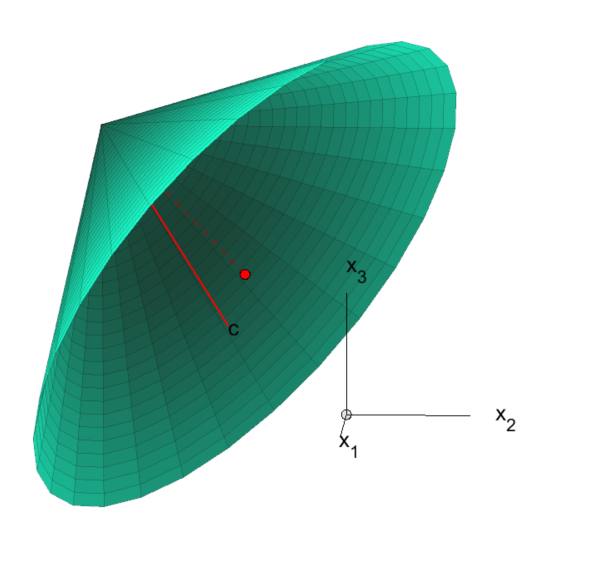
\includegraphics[width=\textwidth]{plotted1}
			\end{subfigure}
			\hfill
			\begin{subfigure}[b]{0.45\textwidth}
				\centering
				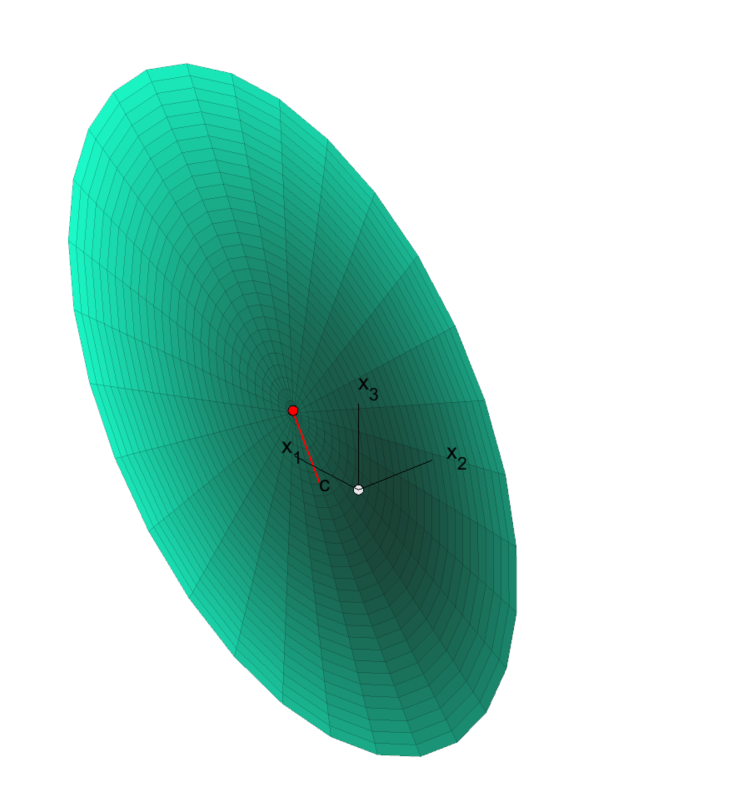
\includegraphics[width=\textwidth]{plotted2}
			\end{subfigure}
			\caption{Cone. Dashed line - centers of level-sets.}
		\end{figure}
		
	\end{flushleft}
\end{frame}





\end{document}
